\documentclass[10pt,a4paper]{article}
\usepackage[utf8]{inputenc}
\usepackage{amsmath}
\usepackage{amsfonts}
\usepackage{amssymb}
\usepackage{graphicx}
\usepackage{bm}
\usepackage{xcolor}
\usepackage{float}
\usepackage[all]{xy}
\title{\vspace{-1in}UR5 / Multi-Camera Calibration}
\author{Gerard Kennedy \& Zheyu Zhang}
\date{}
\begin{document}
\maketitle
\section{Overview}
This document outlines the setup and method for calibrating a multi-camera rig with a UR5 robot arm. 

\section{Problem Formulation\label{problem}}
The task is to develop a pipeline for intrinsic calibration of a multi-camera system, extrinsic calibration of the camera system relative to a global reference frame, and computation of the pose of a UR5 robot and its workspace (a table) relative to the same global reference frame. The global reference frame is defined as the base of the UR5 (see Figure \ref{fig:setup}).

\begin{figure}[H] \centering
	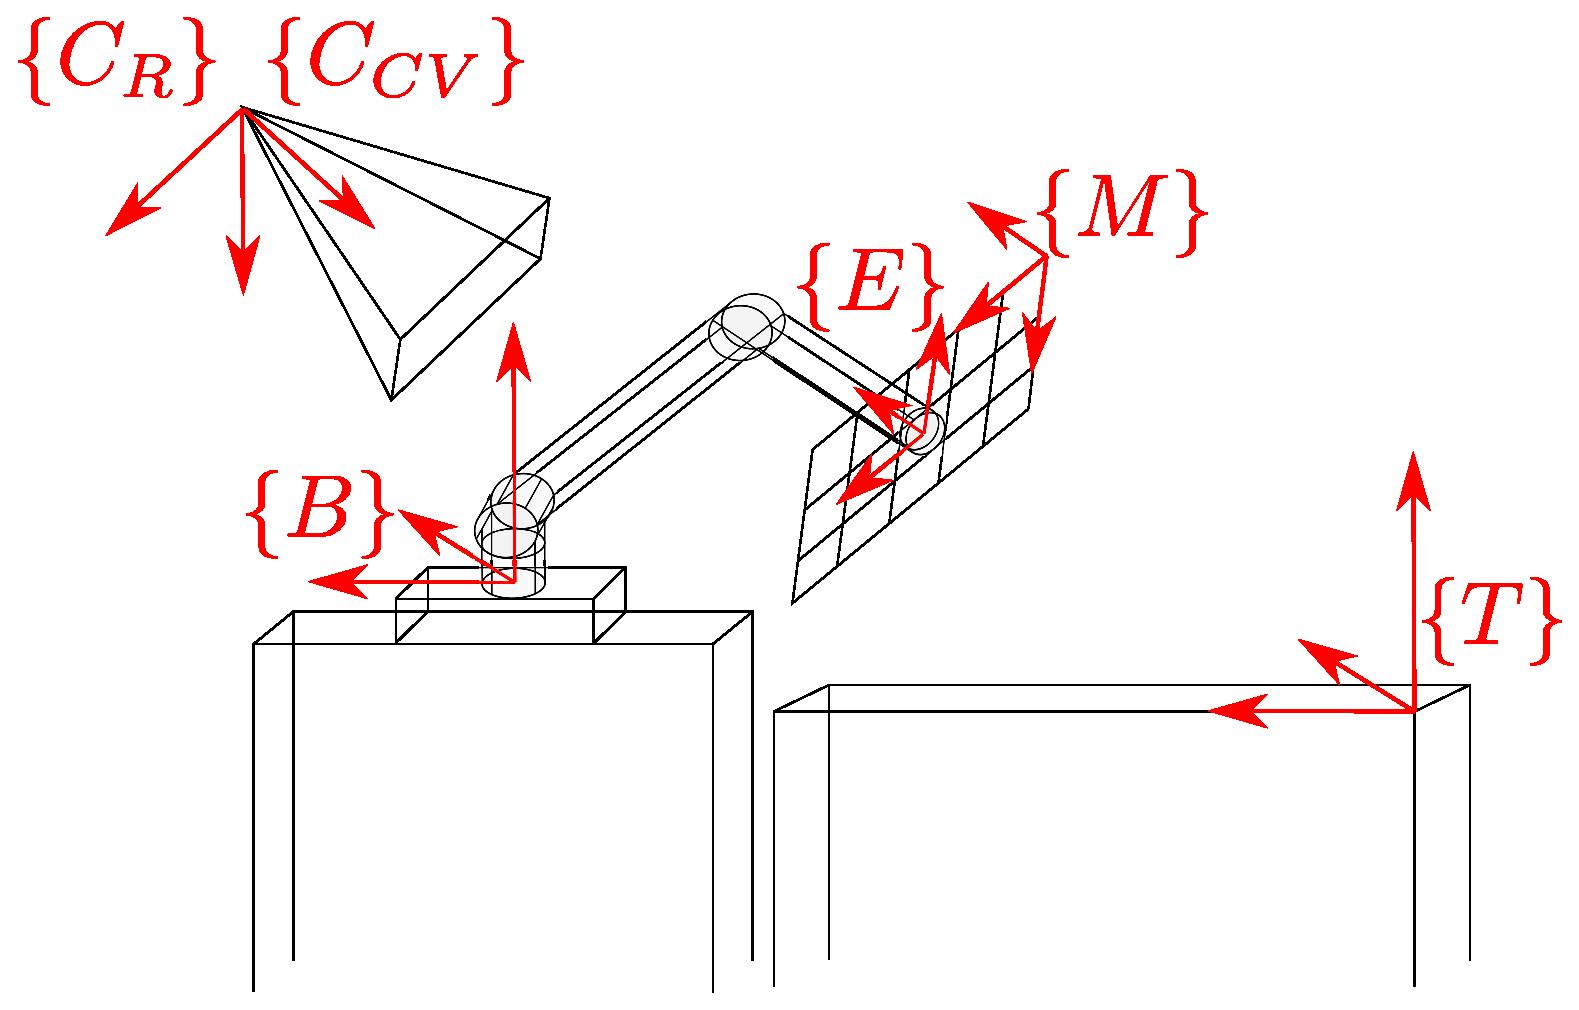
\includegraphics[width=\textwidth]{ur5calib}
	\caption{System setup. $\{C_{CV}\}$ refers to camera pose using the Computer Vision convention, ${C_R}$ refers to camera pose using the Robotics convention, $\{M\}$ refers to the ChAruco Marker board, $\{E\}$ refers to end-effector pose, $\{B\}$ refers to the pose of the UR5 base, and $\{T\}$ refers to the pose of the table.}
	\label{fig:setup}
\end{figure}

\noindent We want to find $\bm{^BX_{C_R},\mbox{} ^BX_T,\mbox{} ^BX_E}$ (i.e. the pose of the camera, table, and end-effector with respect to the base of the UR5). These poses are emphasised in \textbf{bold} in this document.
\\[2ex]

From the setup we know:
\begin{itemize}
	\itemsep0em
	\item $^{M}X_T$ - the pose of the table with respect to the Marker board. This can be found by moving the end-effector so that the calibration board is on the table and measuring the offset.
	\item $^{M}X_{E}$ - the pose of the Marker board with respect to the end-effector when the board is on the table. This is an offset that can be measured, and is related to the provided CAD model.
	\item $^{C_{CV}}X_{C_R}$ - the transformation between the Computer Vision camera pose convention ($z$-axis in the camera focal direction) and the Robotics pose convention ($z$-axis is normal to the ground plane):
	\begin{align*}
	^{C_{CV}}X_{C_R}&=
	\begin{bmatrix}
	0 & -1 & 0 & 0 \\
	0 & 0 & -1 & 0 \\
	1 & 0 & 0 & 0 \\
	0 & 0 & 0 & 1
	\end{bmatrix}
	\end{align*} 
	\item $\bm{^BX_E(\bm{\theta}_i)}$ - the pose of the end-effector with respect to the UR5 base. This can be found via the UR5 forward kinematics  given the UR5 joint angles $\bm{\theta}\in\mathbb{R}^{6\times1}$ at frame $i$.
\end{itemize}

From the extrinsic camera calibration we know:
\begin{itemize}
	\item $^{C_{CV}}X_M$ - the pose of the Marker board with respect to the camera. This is the output of the extrinsic calibration. 
\end{itemize}

\noindent The known and required relative poses are summarised in Figure \ref{fig:frames}.
\begin{figure}[H]
\begin{displaymath}
\xymatrix@C=10em@H=3em{ \{C_{CV}\} \ar[d]|{\color{blue}^{C_{CV}}X_R} & \{T\}  \\
	\{C_R\}  & \{M\} \ar[lu]|{\color{red}\mbox{}^{C_{CV}}X_M} \ar[u]|{\color{blue}^MX_T}\ar[d]|{\color{blue}^MX_E}\\
	\{B\}\ar[ruu]|{\bm{^BX_T}} \ar[u]|{\bm{^BX_{C_R}}} \ar[r]|{\bm{^BX_{E}}} & \{E\} \ }
\label{fig:frames}
\end{displaymath}
\caption{Reference Frames. The 3 required relative poses are shown in \textbf{bold}. The relative poses that can be obtained by measuring an offset or using a known transformation are shown in {\color{blue}blue}. The relative pose provided by the extrinsic calibration is shown in {\color{red}red}.}
\end{figure}



\noindent The remaining poses can be found using the poses listed above. Using the calibration we can find the pose of the camera with respect to the UR5 base $\bm{^BX_{C_R}}$:
\begin{align}
^{C_{CV}}X_E &= \mbox{}^{C_{CV}}X_M\cdot\mbox{}^MX_E\nonumber\\
^EX_{C_R} &= (^{C_{CV}}X_{C_R}^{-1}\cdot\mbox{}^{C_{CV}}X_E)^{-1}\nonumber\\
^BX_{C_R}(\bm{\theta}_i) &= \mbox{}^BX_E(\bm{\theta}_i)\cdot\mbox{}^EX_{C_R}\nonumber\\
\bm{^BX_{C_R}} &= \text{mean}(^BX_{C_R}(\bm{\theta}_i)) \label{eq:C}
\end{align}
Two different approaches can be used to obtain $\bm{^BX_{T}}$ for each image frame. \\
\\
Method 1 (using the forward kinematics):
\begin{align}
^EX_{T_0} &= \mbox{}^MX_E^{-1}\cdot\mbox{}^MX_T \nonumber \\
^BX_{T_0} &=\mbox{}^BX_E\cdot\mbox{}^EX_T \label{eq:1}
\end{align}
Method 2 (using the extrinsic calibration):
\begin{align}
^BX_{T_1} &= \mbox{}^BX_{C_R}\cdot\mbox{}^{C_{R}}X_{C_{CV}}\cdot\mbox{}^{C_{CV}}X_M\cdot\mbox{}^MX_T\label{eq:2}
\end{align}
Using these two Methods we can test the calibration with the following error function.
\begin{align}
E &=||^BX_{T_0} - ^BX_{T_1}||_F
\end{align} 
The final output $\bm{^BX_{T}}$ pose is computed as the mean of Equation (\ref{eq:1}):
\begin{align}
\bm{^BX_{T}} &= \text{mean}(^BX_{T_1})  \label{eq:T}
\end{align} 
The mean poses (Equations (\ref{eq:C}) and (\ref{eq:T}) are obtained by averaging translation values as usual, and averaging rotation over the associated Lie algebras $\mathfrak{so(3)}$. For example, for Equation (\ref{eq:C}):
\begin{align*}
\Omega_i &= \text{log}(^BR_{C}(\bm{\theta}_0)^\top\cdot\mbox{}^BR_{C}(\bm{\theta}_i)), R\in\mathbf{SO(3)}\\
\bar{\Omega} &= \frac{1}{N}\sum_{i=0}^N\Omega_i\\
^B\bar{R}_{C} &=\mbox{} ^BR_{C}(\bm{\theta}_0)\text{exp}(\bar{\Omega})
\end{align*}
Rotation averaging is performed iteratively until convergence using the Karcher (aka Geodesic L2) mean.\\
\\
Figure \ref{fig:calib} shows an example of the ChAruco board attached to the UR5 end-effector.
\begin{figure}[H] \centering
	\includegraphics[width=1.0\textwidth]{exp}
	\caption{Example Setup.}
	\label{fig:calib}
\end{figure}



\end{document}
fix theta, i, hat
dont need averages for rvec, tvec
user input to switch to table calibration